%===================================== CHAP 3 =================================

\chapter{Method}
This chapter will give an insight into why the research is needed and what method used conducting the research. Also, the chapter gives insight into the collection of data,  as well as and who are the participants.

\section{Purpose of the Research} \label{sec:purpose}
%"Describe the reason for doing the research, the topic of interest, why it is important or useful to study this, the specific research question(s) asked and the objectives set. Research without a purpose is unlikely to be good research." (Oates 2005)

%    Write in this section about the following:
%    •	What is the problem? Whose problem is it? Refer to 2-3                good scientific references that confirm for the reader                that this is actually a relevant problem.
%    •	What is done earlier to address this problem? Give 4-5                good references that illustrate the different approaches              taken by other researchers to solve this problem. (you                might also consider to do an in-depth literature review               as part of your autumn project).
%   •	What is wrong with earlier research? Did they not manage              to solve the problem? Why? Why is your approach going to              be better? What new knowledge do you plan to add?
%    •	Summarize with a list of clearly defined research                     questions. One main question and 2-3 sub-questions                    related to the main question. Note that the sub-questions             should contribute to answer the main question.

This research constist of two phases; (1) the projects thesis in the fall: which will include examining of the problem space and give the research questions for the following master thesis; and (2) the master thesis the following spring: which has the interntion to answer the questions purposed by the project thesis.

The domain of this project consists of several different subjects. The Case chosen is a construction project. The researcher's origin is software development, and the problem discussed is also compared with the ICT-industry. The reason for this comparison is the use of APM in both industries. When comparing the two industries, the comparison is justified; Both have experienced problems in meeting budgets and delivering at the planned deadline and function, as well as experienced increased complexity. This problem is materialized in extensive documentation, change of requirements during production, failing to fix errors, and problems delivering a product that meets the requirements of the users. APM is mainly a structured way for the managers to direct the interaction between actors and participants in the project; thus, cooperation and interaction are a part of the problem space. In addition to using APM, the case object is also utilizing software supporting both management and cooperation. 

The variety in problem space makes this research important, not only for the CI-industry and the ICT-industry. Other industries utilizing digital tools or Agile solving complex engineering problems or interaction, will find this research relevant. 

Prior research relevant for this project is mainly the paper describing the construction of the Peter B. Lewis Building (PLB), where 3-D modeling was first introduced \cite{frank_gehry}. 3-D modeling was used both to manage the complexity of the installation, but also led to increased cooperation between different parties within the project. Even though the PLB-project showed promising results in means of cooperation and interaction, the introduction of 3-D modeling was not a single solution to the problem. 

Relevant is also the book \textit{Lean methodology in design and construction} \cite{lean_i_praksis} describes the making of the Bergen Academy of Art and Design-building, where Lean was one of the essential strategies. The managers of the project wrote this book; hence, the descriptions given are sufficient critical but still relevant as a cite for the project. 

Notable literature relevant in this research is, among others, the research in the topic of contractors, and how different aspects of contracts influence cooperation \cite{miller2002harmonization, zaghloul2003construction}. The Rolfsen \& Bruvik paper is discussing the trust in construction project teams \cite{rolfsen}. Common for these three papers is that they do not consider the complete problem domain; they lack the inclusion of APM and digitalization. Moreover, the Monplaisir paper concerning CSCW in Agile Manufacturing \cite{monplaisir2002enhancing} is, therefore, more relevant but lack the problem domain of the CI. 

The motivation for this rearch is to examine a project utilizing Lean in project management, to face the problems mentioned. Furthermore, looking at how a project make use of digital tools, aiding Lean has not been examined before. Taking experience from the ICT-industry, and the use of computer-aided agile development management is also desirable, as well as looking at the problem from a different perspective.

This project, therefore, aims to examine a case using Lean methodology, where digital tools are utilized to support both the methodology as well as cooperation and interaction between different actors.

{\noindent \bf $RQ1$: Is the use of Lean in the LSB-project simply a project management buzz?} \\
{\bf $RQ2$: What can be done contributing to the use of Lean and CSCW in the LSB-project?}

\section{Contributions}
%"Describe the outcomes of research, especially your contribution to knowledge about your subject area. Your contribution can be an answer to your original research question( s) but can also include unexpected findings. For example, you and the academic community might learn something about a particular research strategy as a result of your research. Your thesis, dissertation, conference paper or journal article is also a product of your research. For those research projects that involve design and creation, a new computer-based product or new development method could also be a product of your research." (Oates 2005)

%Types of research products: 1) new or improved evidence; 2) new or improved methodology; 3) new or improved analysis; 4) new or improved concepts or theories; 5) new or improved computer-based product.

%Write in this section about the following:
%•	What will be your research contribution? Which of the          four types above?
%•	How and why will it be better than earlier contributions?

The main contribution of the study is the knowledge of how participants in a Norwegian CI project adapt to new software tools aiding Lean Construction management. The project thesis has two valuable contributions: (1) the literature review; and (2) guidance as to where to target the research in the master thesis. The master thesis will consist of data collection and the analysis of the data, where the result of the analysis adds to the main contribution. 

There is little to none studies of this particular problem, and therefore, it stands as a single contribution to the specific field. The use and implementation of new software are considered a significant field of study in computer science, but using this knowledge in the CI will, consequently, give insights they never have and rigorously wants, given the will for digitalization; hence, this study is desirable.

\section{Research Method}
%"Describe the sequence of activities undertaken in any research project. The process involves identifying one or more research topics, establishing a conceptual framework (the way you choose to think about your research topic), the selection and use of a research strategy and data generation methods, the analysis of data and the drawing of conclusions, including recognizing any limitations in your own research. As explained already, the process should be carried out systematically if the research is to be accepted as rigorous."
%Write here your (See the figure below from Oates 2005):
%•	Research strategy (survey, case study, action research,        experiment, design etc.)
%•	Is this mixed-method? Then you can have different              strategies for different steps in the design.
%•	Data generation methods (interview, focus group,               observation, documents etc.)
%•	You can have more than one data generation method for          each strategy.
%• 	Data analysis methods (qualitative or quantitative.)

\begin{figure}
    \begin{center}
        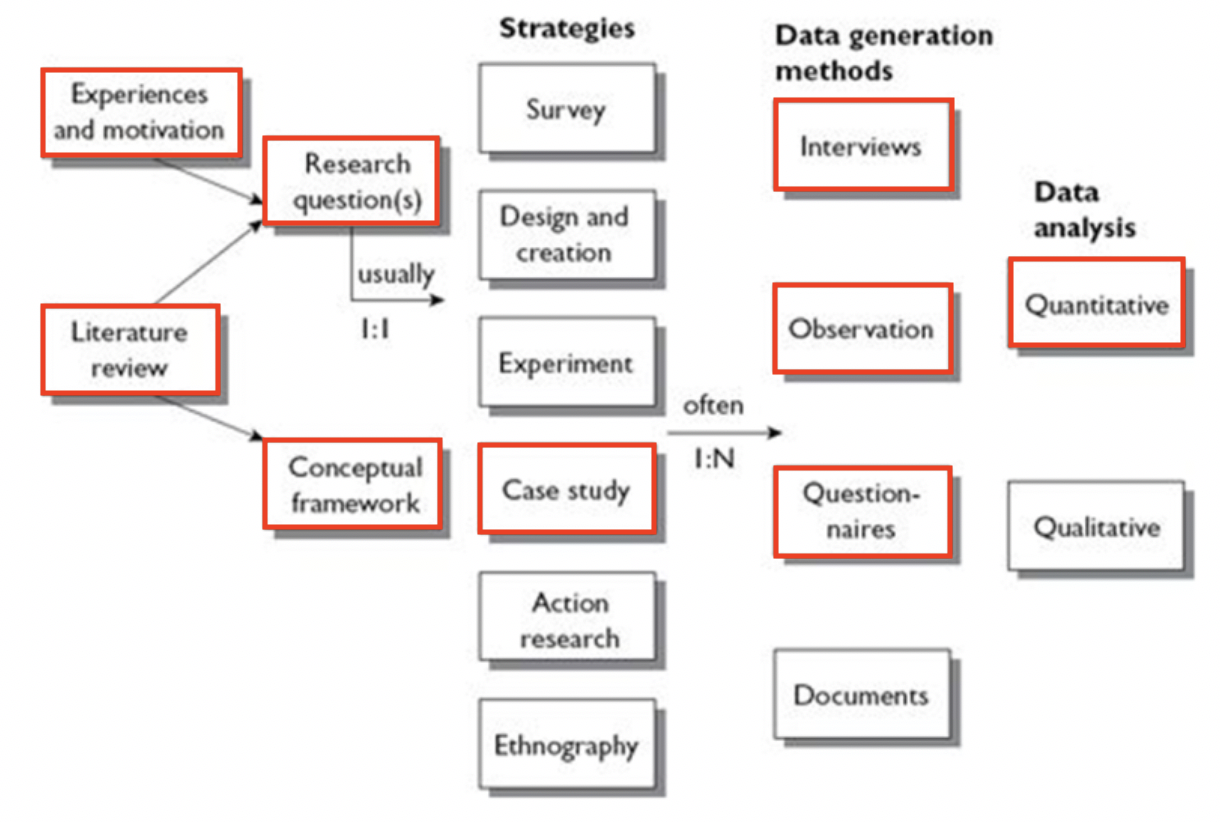
\includegraphics[width=0.8\textwidth]{fig/empirisk_studie.png}
        \caption{The research process used, marked with methods applied in the research.}
    \end{center}
    \label{fig:my_label}
\end{figure}

This project originated in an interest in Software methodology, and how software aids productivity and cooperation in different parts of society. The projects formed when Patrick Stormo Hjerpseth, who is the Project Lead in Digitalization at the LSB-project, gave a tip regarding writing a master thesis about the LSB-project.

The project started with a literature review, providing a knowledgeable background for the project. Based on the literature review, one could see a clear correlation between software engineering (SE) 30 years ago and the construction engineering (CE) of today, as mentioned in the \nameref{sec:purpose} section. To identify how these problems can be faced in a project, using agile management methods and CSCW, the master thesis is planning a case study-strategy. The case studied is the LSB-project. 

In this project thesis the research will consist of a minor empirical study, utilizing observation and interviews as data generators. This research will hopefully give insights that will narrow the focus of the master thesis. The interviews was conducted with a semi-structured approach, with some standardized questions, listed in Appendix \ref{apx:interview_guide}, for every interview. The list of interviewees can be seen in table \ref{tab:paticipants}. 

\begin{table}[]
    \begin{center}
        \begin{tabular}{@{}lll@{}}
        \toprule
        \textbf{Interviewee} & \textbf{Function}          & \textbf{Gender} \\ \midrule
        1                    & Assistant Project Director \& Project Manager & Male            \\
        2                    & Assistant Project Manager  & Male            \\
        Total interviews     & \multicolumn{2}{r}{2}                        \\ \bottomrule
        \end{tabular}
        \caption{Overview over interviews in the project thesis.}
        \label{tab:paticipants}
    \end{center}
\end{table}

The observations was done over a two days period, on the project office, where different meetings was observed. The list of interviews can be seen in table \ref{tab:observations}. Adding to the observations, talking to the managers and PLs, when on site, gave valuable insight into how the project is run.

\begin{table}[]
    \begin{center}
        \begin{tabular}{@{}ll@{}}
        \toprule
        \textbf{Obervation} & \textbf{Meeting}       \\ \midrule
        1                   & Blackboard-meeting     \\
        2                   & Table-test meeting     \\
        3                   & Digitalization-meeting \\
        4                   & BIM and dRofus introduction \\
        Total observations  & \multicolumn{1}{r}{4}  \\ \bottomrule
        \end{tabular}
        \caption{List of observations conducted in the project thesis.}
        \label{tab:observations}
    \end{center}
\end{table}

\section{Participants}
%"These include those whom you directly involve in your research, for example by interviewing them or observing them, and also those who are indirectly involved, such as the editors to whom you submit a research paper. It is important that you deal with all these people legally and ethically, that is, you do not do anything that might annoy them or cause them harm (physically, mentally or socially). You yourself as a researcher are also a research participant. As we shall see later, for some types of research, researchers are expected to be objective and remain largely unseen in the reporting of their research, whereas in other types of research the researchers are open about their feelings and how their presence influenced the other participants and the research situation."
%You need to clarify the following:
%•	Who are the informants? How do you plan to recruit them?
%•	If you want to collect data you should take care of the ethical       issues. E.g. 1) you should get approval from NSD before you           start collecting data, 2) you should have users sign informed         consent forms, 3) you should make sure you don't share                person-related data (e.g. you cannot have this data on Google         doc!).
%•	Don't underestimate use recruitment. It is often the part of the       research that shows to be the most problematic! Get started           early.
%•	Who are the researchers?
%•	Be specific who will do what in the project.

The project researcher, Morten Bujordet, is involved in the project, creating the plans, and conducting the research.
	 
Supervising the project is Eric Monteiro. Monteiro is contributing with experience in research in the implementation and use of new digital tools in large scale, as welle as complex organizations. 

Furthermore, Statsbygg, as the manager, has an interest in the project: giving access to the participants in the study. With Patrick Stormo Hjerpseth as the point of contact.
	 
In the research, the actors using the digital software in the project design will be an aim for the data collection. All personal information gathered will, safely, be stored in a GDPR-compliant Cloud Service, served by NTNU. In the final report, no personal information will be published, and all actors in the data collection will be anonymized.


\section{Research Paradigm}
%"A pattern or model or shared way of thinking. Managers sometimes talk of the need for a ‘paradigm shift’ to mean that a new way of thinking is required. In computing, we talk about programming language paradigms, for example, a group of languages that share a set of characteristics, such as the object-oriented paradigm (for example, Smalltalk and C + +). Here we are concerned with the philosophical paradigms of research. Any piece of research will have an underlying paradigm. We have noted already that different academic communities and individuals have different ideas about the kinds of research questions to ask and the process by which to answer them because they have different views about the nature of the world we live in and therefore about how we might investigate it. These different views stem from different philosophical paradigms. We shall look at three such paradigms: ‘positivism’, interpretivism’ and ‘critical research’ – each will be explained later."

The research is adopting a Case Study-strategy of a single case object. Data is generated using, as mentioned, two methods: interviews, and a questionnaire. This study is related to the positivism paradigm — the use of empirical observation of the participants and a desire to identify how they act on the new software used. Using interviews can lead to not being objective as all collection of data is done in interaction with the participants. This yields a qualitative collection of data. The purpose of this project thesis is to identify the problems worth exploring in the master thesis. The not to objective study is, therefore, accepted.

\cleardoublepage